\documentclass{article}

\def \lastexercisenumber {0}

\usepackage[utf8]{inputenc}
\usepackage{fullpage}
\usepackage{amsmath, amssymb, amsfonts, amsthm}
\usepackage{bbm}
\usepackage{mathtools}
\usepackage{twoopt}

% special letters:

\newcommand{\N}{\mathbb{N}}
\newcommand{\Z}{\mathbb{Z}}
\newcommand{\Q}{\mathbb{Q}}
\newcommand{\R}{\mathbb{R}}
\newcommand{\C}{\mathbb{C}}
\newcommand{\K}{\mathbb{K}}
\newcommand{\T}{\mathbb{T}}
\newcommand{\E}{\mathbb{E}}
\newcommand{\V}{\mathbb{V}}
\renewcommand{\S}{\mathbb{S}}
\renewcommand{\P}{\mathbb{P}}
\newcommand{\1}{\mathbbm{1}}

% quantors:

\newcommand{\Forall}{\forall \,}
\newcommand{\Exists}{\exists \,}
\newcommand{\ExistsOnlyOne}{\exists! \,}
\newcommand{\nExists}{\nexists \,}
\newcommand{\ForAlmostAll}{\forall^\infty \,}

% MISC symbols:

\newcommand{\landau}{{\scriptstyle \mathcal{O}}}
\newcommand{\Landau}{\mathcal{O}}


\newcommand{\eps}{\mathrm{eps}}

% graphics in a box:

\newcommandtwoopt
{\includegraphicsboxed}[3][][]
{
  \begin{figure}[!h]
    \begin{boxedin}
      \ifthenelse{\isempty{#1}}
      {
        \begin{center}
          \includegraphics[width = 0.75 \textwidth]{#3}
          \label{fig:#2}
        \end{center}
      }{
        \begin{center}
          \includegraphics[width = 0.75 \textwidth]{#3}
          \caption{#1}
          \label{fig:#2}
        \end{center}
      }
    \end{boxedin}
  \end{figure}
}

% braces:

\newcommand{\pbraces}[1]{{\left  ( #1 \right  )}}
\newcommand{\bbraces}[1]{{\left  [ #1 \right  ]}}
\newcommand{\Bbraces}[1]{{\left \{ #1 \right \}}}
\newcommand{\vbraces}[1]{{\left  | #1 \right  |}}
\newcommand{\Vbraces}[1]{{\left \| #1 \right \|}}
\newcommand{\abraces}[1]{{\left \langle #1 \right \rangle}}
\newcommand{\round}[1]{\bbraces{#1}}

\newcommand
{\floorbraces}[1]
{{\left \lfloor #1 \right \rfloor}}

\newcommand
{\ceilbraces} [1]
{{\left \lceil  #1 \right \rceil }}

% special functions:

\newcommand{\norm}  [2][]{\Vbraces{#2}_{#1}}
\newcommand{\diam}  [2][]{\mathrm{diam}_{#1} \: #2}
\newcommand{\diag}  [1]{\mathrm{diag} \: #1}
\newcommand{\dist}  [1]{\mathrm{dist} \: #1}
\newcommand{\mean}  [1]{\mathrm{mean} \: #1}
\newcommand{\erf}   [1]{\mathrm{erf} \: #1}
\newcommand{\id}    [1]{\mathrm{id} \: #1}
\newcommand{\sgn}   [1]{\mathrm{sgn} \: #1}
\newcommand{\supp}  [1]{\mathrm{supp} \: #1}
\newcommand{\arsinh}[1]{\mathrm{arsinh} \: #1}
\newcommand{\arcosh}[1]{\mathrm{arcosh} \: #1}
\newcommand{\artanh}[1]{\mathrm{artanh} \: #1}
\newcommand{\card}  [1]{\mathrm{card} \: #1}
\newcommand{\Span}  [1]{\mathrm{span} \: #1}
\newcommand{\Aut}   [1]{\mathrm{Aut} \: #1}
\newcommand{\End}   [1]{\mathrm{End} \: #1}
\newcommand{\ggT}   [1]{\mathrm{ggT} \: #1}
\newcommand{\kgV}   [1]{\mathrm{kgV} \: #1}
\newcommand{\ord}   [1]{\mathrm{ord} \: #1}
\newcommand{\grad}  [1]{\mathrm{grad} \: #1}
\newcommand{\ran}   [1]{\mathrm{ran} \: #1}
\newcommand{\graph} [1]{\mathrm{graph} \: #1}
\newcommand{\Inv}   [1]{\mathrm{Inv} \: #1}
\newcommand{\pv}    [1]{\mathrm{pv} \: #1}
\newcommand{\GL}    [1]{\mathrm{GL} \: #1}
\newcommand{\Mod}{\mathrm{Mod} \:}
\newcommand{\Th}{\mathrm{Th} \:}
\newcommand{\Char}{\mathrm{char}}
\newcommand{\At}{\mathrm{At}}
\newcommand{\Ob}{\mathrm{Ob}}
\newcommand{\Hom}{\mathrm{Hom}}
\newcommand{\orthogonal}[3][]{#2 ~\bot_{#1}~ #3}
\newcommand{\Rang}{\mathrm{Rang}}
\newcommand{\NIL}{\mathrm{NIL}}
\newcommand{\Res}{\mathrm{Res}}
\newcommand{\lxor}{\dot \lor}
\newcommand{\Div}{\mathrm{div} \:}
\newcommand{\meas}{\mathrm{meas} \:}

% fractions:

\newcommand{\Frac}[2]{\frac{1}{#1} \pbraces{#2}}
\newcommand{\nfrac}[2]{\nicefrac{#1}{#2}}

% derivatives & integrals:

\newcommandtwoopt
{\Int}[4][][]
{\int_{#1}^{#2} #3 ~\mathrm{d} #4}

\newcommandtwoopt
{\derivative}[3][][]
{
  \frac
  {\mathrm{d}^{#1} #2}
  {\mathrm{d} #3^{#1}}
}

\newcommandtwoopt
{\pderivative}[3][][]
{
  \frac
  {\partial^{#1} #2}
  {\partial #3^{#1}}
}

\newcommand
{\primeprime}
{{\prime \prime}}

\newcommand
{\primeprimeprime}
{{\prime \prime \prime}}

% Text:

\newcommand{\Quote}[1]{\glqq #1\grqq{}}
\newcommand{\Text}[1]{{\text{#1}}}
\newcommand{\fastueberall}{\text{f.ü.}}
\newcommand{\fastsicher}{\text{f.s.}}

% -------------------------------- %
% amsthm-stuff:

\theoremstyle{definition}

% numbered theorems
\newtheorem{theorem}{Satz}
\newtheorem{lemma}{Lemma}
\newtheorem{corollary}{Korollar}
\newtheorem{proposition}{Proposition}
\newtheorem{remark}{Bemerkung}
\newtheorem{definition}{Definition}
\newtheorem{example}{Beispiel}

% unnumbered theorems
\newtheorem*{theorem*}{Satz}
\newtheorem*{lemma*}{Lemma}
\newtheorem*{corollary*}{Korollar}
\newtheorem*{proposition*}{Proposition}
\newtheorem*{remark*}{Bemerkung}
\newtheorem*{definition*}{Definition}
\newtheorem*{example*}{Beispiel}

% Please define this stuff in project ("main.tex"):

% \def \lastexercisenumber {...}
% This will be 0 by default

% \setcounter{section}{...}
% This will be 0 by default
% and hence, completely ignored

\ifnum \thesection = 0
{\newtheorem{exercise}{Aufgabe}}
\else
{\newtheorem{exercise}{Aufgabe}[section]}
\fi

\ifdef
{\lastexercisenumber}
{\setcounter{exercise}{\lastexercisenumber}}

\newcommand{\solution}
{
    \renewcommand{\proofname}{Lösung}
    \renewcommand{\qedsymbol}{}
    \proof
}

\renewcommand{\proofname}{Beweis}

% -------------------------------- %
% environment zum einkasteln:

% dickere vertical lines
\newcolumntype
{x}
[1]
{!{\centering\arraybackslash\vrule width #1}}

% environment selbst (the big cheese)
\newenvironment
{boxedin}
{
  \begin{tabular}
  {
    x{1 pt}
    p{\textwidth}
    x{1 pt}
  }
  \Xhline
  {2 \arrayrulewidth}
}
{
  \\
  \Xhline{2 \arrayrulewidth}
  \end{tabular}
}

% -------------------------------- %
% MISC "Ein-Deutschungen"

\renewcommand
{\figurename}
{Abbildung}

\renewcommand
{\tablename}
{Tabelle}

% -------------------------------- %

% ---------------------------------------------------------------- %
% https://www.overleaf.com/learn/latex/Code_listing

\definecolor{codegreen} {rgb}{0, 0.6, 0}
\definecolor{codegray}    {rgb}{0.5, 0.5, 0.5}
\definecolor{codepurple}{rgb}{0.58, 0, 0.82}
\definecolor{backcolour}{rgb}{0.95, 0.95, 0.92}

\lstdefinestyle{overleaf}
{
    backgroundcolor = \color{backcolour},
    commentstyle = \color{codegreen},
    keywordstyle = \color{magenta},
    numberstyle = \tiny\color{codegray},
    stringstyle = \color{codepurple},
    basicstyle = \ttfamily \footnotesize,
    breakatwhitespace = false,
    breaklines = true,
    captionpos = b,
    keepspaces = true,
    numbers = left,
    numbersep = 5pt,
    showspaces = false,
    showstringspaces = false,
    showtabs = false,
    tabsize = 2
}

% ---------------------------------------------------------------- %
% https://en.wikibooks.org/wiki/LaTeX/Source_Code_Listings

\lstdefinestyle{customc}
{
    belowcaptionskip = 1 \baselineskip,
    breaklines = true,
    frame = L,
    xleftmargin = \parindent,
    language = C,
    showstringspaces = false,
    basicstyle = \footnotesize \ttfamily,
    keywordstyle = \bfseries \color{green!40!black},
    commentstyle = \itshape \color{purple!40!black},
    identifierstyle = \color{blue},
    stringstyle = \color{orange},
}

\lstdefinestyle{customasm}
{
    belowcaptionskip = 1 \baselineskip,
    frame = L,
    xleftmargin = \parindent,
    language = [x86masm] Assembler,
    basicstyle = \footnotesize\ttfamily,
    commentstyle = \itshape\color{purple!40!black},
}

% ---------------------------------------------------------------- %
% https://tex.stackexchange.com/questions/235731/listings-syntax-for-literate

\definecolor{maroon}        {cmyk}{0, 0.87, 0.68, 0.32}
\definecolor{halfgray}      {gray}{0.55}
\definecolor{ipython_frame} {RGB}{207, 207, 207}
\definecolor{ipython_bg}    {RGB}{247, 247, 247}
\definecolor{ipython_red}   {RGB}{186, 33, 33}
\definecolor{ipython_green} {RGB}{0, 128, 0}
\definecolor{ipython_cyan}  {RGB}{64, 128, 128}
\definecolor{ipython_purple}{RGB}{170, 34, 255}

\lstdefinestyle{stackexchangePython}
{
    breaklines = true,
    %
    extendedchars = true,
    literate =
    {á}{{\' a}} 1 {é}{{\' e}} 1 {í}{{\' i}} 1 {ó}{{\' o}} 1 {ú}{{\' u}} 1
    {Á}{{\' A}} 1 {É}{{\' E}} 1 {Í}{{\' I}} 1 {Ó}{{\' O}} 1 {Ú}{{\' U}} 1
    {à}{{\` a}} 1 {è}{{\` e}} 1 {ì}{{\` i}} 1 {ò}{{\` o}} 1 {ù}{{\` u}} 1
    {À}{{\` A}} 1 {È}{{\' E}} 1 {Ì}{{\` I}} 1 {Ò}{{\` O}} 1 {Ù}{{\` U}} 1
    {ä}{{\" a}} 1 {ë}{{\" e}} 1 {ï}{{\" i}} 1 {ö}{{\" o}} 1 {ü}{{\" u}} 1
    {Ä}{{\" A}} 1 {Ë}{{\" E}} 1 {Ï}{{\" I}} 1 {Ö}{{\" O}} 1 {Ü}{{\" U}} 1
    {â}{{\^ a}} 1 {ê}{{\^ e}} 1 {î}{{\^ i}} 1 {ô}{{\^ o}} 1 {û}{{\^ u}} 1
    {Â}{{\^ A}} 1 {Ê}{{\^ E}} 1 {Î}{{\^ I}} 1 {Ô}{{\^ O}} 1 {Û}{{\^ U}} 1
    {œ}{{\oe}}  1 {Œ}{{\OE}}  1 {æ}{{\ae}}  1 {Æ}{{\AE}}  1 {ß}{{\ss}}  1
    {ç}{{\c c}} 1 {Ç}{{\c C}} 1 {ø}{{\o}} 1 {å}{{\r a}} 1 {Å}{{\r A}} 1
    {€}{{\EUR}} 1 {£}{{\pounds}} 1
}


% Python definition (c) 1998 Michael Weber
% Additional definitions (2013) Alexis Dimitriadis
% modified by me (should not have empty lines)

\lstdefinelanguage{iPython}{
    morekeywords = {access, and, break, class, continue, def, del, elif, else, except, exec, finally, for, from, global, if, import, in, is, lambda, not, or, pass, print, raise, return, try, while}, %
    %
    % Built-ins
    morekeywords = [2]{abs, all, any, basestring, bin, bool, bytearray, callable, chr, classmethod, cmp, compile, complex, delattr, dict, dir, divmod, enumerate, eval, execfile, file, filter, float, format, frozenset, getattr, globals, hasattr, hash, help, hex, id, input, int, isinstance, issubclass, iter, len, list, locals, long, map, max, memoryview, min, next, object, oct, open, ord, pow, property, range, raw_input, reduce, reload, repr, reversed, round, set, setattr, slice, sorted, staticmethod, str, sum, super, tuple, type, unichr, unicode, vars, xrange, zip, apply, buffer, coerce, intern}, %
    %
    sensitive = true, %
    morecomment = [l] \#, %
    morestring = [b]', %
    morestring = [b]", %
    %
    morestring = [s]{'''}{'''}, % used for documentation text (mulitiline strings)
    morestring = [s]{"""}{"""}, % added by Philipp Matthias Hahn
    %
    morestring = [s]{r'}{'},     % `raw' strings
    morestring = [s]{r"}{"},     %
    morestring = [s]{r'''}{'''}, %
    morestring = [s]{r"""}{"""}, %
    morestring = [s]{u'}{'},     % unicode strings
    morestring = [s]{u"}{"},     %
    morestring = [s]{u'''}{'''}, %
    morestring = [s]{u"""}{"""}, %
    %
    % {replace}{replacement}{lenght of replace}
    % *{-}{-}{1} will not replace in comments and so on
    literate = 
    {á}{{\' a}} 1 {é}{{\' e}} 1 {í}{{\' i}} 1 {ó}{{\' o}} 1 {ú}{{\' u}} 1
    {Á}{{\' A}} 1 {É}{{\' E}} 1 {Í}{{\' I}} 1 {Ó}{{\' O}} 1 {Ú}{{\' U}} 1
    {à}{{\` a}} 1 {è}{{\` e}} 1 {ì}{{\` i}} 1 {ò}{{\` o}} 1 {ù}{{\` u}} 1
    {À}{{\` A}} 1 {È}{{\' E}} 1 {Ì}{{\` I}} 1 {Ò}{{\` O}} 1 {Ù}{{\` U}} 1
    {ä}{{\" a}} 1 {ë}{{\" e}} 1 {ï}{{\" i}} 1 {ö}{{\" o}} 1 {ü}{{\" u}} 1
    {Ä}{{\" A}} 1 {Ë}{{\" E}} 1 {Ï}{{\" I}} 1 {Ö}{{\" O}} 1 {Ü}{{\" U}} 1
    {â}{{\^ a}} 1 {ê}{{\^ e}} 1 {î}{{\^ i}} 1 {ô}{{\^ o}} 1 {û}{{\^ u}} 1
    {Â}{{\^ A}} 1 {Ê}{{\^ E}} 1 {Î}{{\^ I}} 1 {Ô}{{\^ O}} 1 {Û}{{\^ U}} 1
    {œ}{{\oe}}  1 {Œ}{{\OE}}  1 {æ}{{\ae}}  1 {Æ}{{\AE}}  1 {ß}{{\ss}}  1
    {ç}{{\c c}} 1 {Ç}{{\c C}} 1 {ø}{{\o}} 1 {å}{{\r a}} 1 {Å}{{\r A}} 1
    {€}{{\EUR}} 1 {£}{{\pounds}} 1
    %
    {^}{{{\color{ipython_purple}\^ {}}}} 1
    { = }{{{\color{ipython_purple} = }}} 1
    %
    {+}{{{\color{ipython_purple}+}}} 1
    {*}{{{\color{ipython_purple}$^\ast$}}} 1
    {/}{{{\color{ipython_purple}/}}} 1
    %
    {+=}{{{+=}}} 1
    {-=}{{{-=}}} 1
    {*=}{{{$^\ast$ = }}} 1
    {/=}{{{/=}}} 1,
    literate = 
    *{-}{{{\color{ipython_purple} -}}} 1
     {?}{{{\color{ipython_purple} ?}}} 1,
    %
    identifierstyle = \color{black}\ttfamily,
    commentstyle = \color{ipython_cyan}\ttfamily,
    stringstyle = \color{ipython_red}\ttfamily,
    keepspaces = true,
    showspaces = false,
    showstringspaces = false,
    %
    rulecolor = \color{ipython_frame},
    frame = single,
    frameround = {t}{t}{t}{t},
    framexleftmargin = 6mm,
    numbers = left,
    numberstyle = \tiny\color{halfgray},
    %
    %
    backgroundcolor = \color{ipython_bg},
    % extendedchars = true,
    basicstyle = \scriptsize,
    keywordstyle = \color{ipython_green}\ttfamily,
}

% ---------------------------------------------------------------- %
% https://tex.stackexchange.com/questions/417884/colour-r-code-to-match-knitr-theme-using-listings-minted-or-other

\geometry{verbose, tmargin = 2.5cm, bmargin = 2.5cm, lmargin = 2.5cm, rmargin = 2.5cm}

\definecolor{backgroundCol}  {rgb}{.97, .97, .97}
\definecolor{commentstyleCol}{rgb}{0.678, 0.584, 0.686}
\definecolor{keywordstyleCol}{rgb}{0.737, 0.353, 0.396}
\definecolor{stringstyleCol} {rgb}{0.192, 0.494, 0.8}
\definecolor{NumCol}         {rgb}{0.686, 0.059, 0.569}
\definecolor{basicstyleCol}  {rgb}{0.345, 0.345, 0.345}

\lstdefinestyle{stackexchangeR}
{
    language = R,                                        % the language of the code
    basicstyle = \small \ttfamily \color{basicstyleCol}, % the size of the fonts that are used for the code
    % numbers = left,                                      % where to put the line-numbers
    numberstyle = \color{green},                         % the style that is used for the line-numbers
    stepnumber = 1,                                      % the step between two line-numbers. If it is 1, each line will be numbered
    numbersep = 5pt,                                     % how far the line-numbers are from the code
    backgroundcolor = \color{backgroundCol},             % choose the background color. You must add \usepackage{color}
    showspaces = false,                                  % show spaces adding particular underscores
    showstringspaces = false,                            % underline spaces within strings
    showtabs = false,                                    % show tabs within strings adding particular underscores
    % frame = single,                                      % adds a frame around the code
    % rulecolor = \color{white},                           % if not set, the frame-color may be changed on line-breaks within not-black text (e.g. commens (green here))
    tabsize = 2,                                         % sets default tabsize to 2 spaces
    captionpos = b,                                      % sets the caption-position to bottom
    breaklines = true,                                   % sets automatic line breaking
    breakatwhitespace = false,                           % sets if automatic breaks should only happen at whitespace
    keywordstyle = \color{keywordstyleCol},              % keyword style
    commentstyle = \color{commentstyleCol},              % comment style
    stringstyle = \color{stringstyleCol},                % string literal style
    literate = %
    *{0}{{{\color{NumCol} 0}}} 1
     {1}{{{\color{NumCol} 1}}} 1
     {2}{{{\color{NumCol} 2}}} 1
     {3}{{{\color{NumCol} 3}}} 1
     {4}{{{\color{NumCol} 4}}} 1
     {5}{{{\color{NumCol} 5}}} 1
     {6}{{{\color{NumCol} 6}}} 1
     {7}{{{\color{NumCol} 7}}} 1
     {8}{{{\color{NumCol} 8}}} 1
     {9}{{{\color{NumCol} 9}}} 1
}

% ---------------------------------------------------------------- %
% Fundament Mathematik

\lstdefinestyle{fundament}{basicstyle = \ttfamily}

% ---------------------------------------------------------------- %


\parskip 0pt
\parindent 0pt

\title
{
  Maß- und Wahrscheinlichkeitstheorie 2 - Übung 12\\
  \vspace{4pt}
  \normalsize
  \textit{12. UE am 15.01.2020}
}
\author
{
  Richard Weiss       \and
  Florian Schager     \and
  Christian Sallinger \and
  Fabian Zehetgruber  \and
  Paul Winkler        \and
  Christian Göth
}
\date{}

\begin{document}

\maketitle

\begin{align*}
  \Phi:
  \overline{\R} \to [0, 1]:
  x \mapsto \frac{1}{\sqrt{2 \pi}} \Int[-\infty][x]{e^\frac{-t^2}{2}}{t}
\end{align*}

\begin{algebraUE}{384}
Sei $R$ der Polynomring $(\Z/5\Z)[t]$, und sei $U \subseteq R$ der kleinste
Unterring mit $1$ von $R$, der das Polynom $t^5$ enthält. Geben Sie ein Polynom
$p(x) \in U[x]$ an, welches in $R$ die Nullstelle $t$ hat. (Wenn Ihnen das zu
leicht ist: Finden Sie so ein Polynom, welches in $U[x]$ irreduzibel ist.)
\end{algebraUE}

\begin{solution}
\begin{align*}
  U &= \left\{\sum_{k = 0}^na_kt^{5k}: n \in \N, a_k \in \Z/5\Z, k = 0,\dots,n\right\} \\
  p(x) &= x^5 - t^5.
\end{align*}
Über $R$ ist $t$ die einzige Nullstelle von $p(x)$. Polynomdivision liefert
\begin{align*}
  (x^5-t^5):(x-t) = x^4 + tx^3 + t^2x^2 + t^3x + t^4.
\end{align*}

Da jedes lineare Polynom
eine Nullstelle in $U$ besitzt, bleibt als einzige Möglichkeit zur Reduktion
in irreduzible Faktoren die Faktorisierung in ein Polynom $q(x)$ 2-ten und ein Polynom
$r(x)$ 3-ten Grades übrig (o.B.d.A. normiert).
Angenommen
\begin{align*}
  p(x) &= q(x)r(x) = (x^3 + bx^2 + cx + d)(x^2 + fx + g) \\
  &= x^5 + (f + b)x^4 + (g + bf + c)x^3 +(bg + cf + d)x^2 + (cg + df)x + dg.
\end{align*}

\end{solution}

\begin{algebraUE}{386}

  \begin{itemize}
      \item[1.] Sei $p \in \mathbb{P}, k, n \in \mathbb{N}, n \geq 1.$ Dann ist $\varphi: a \mapsto a^p$ ein Automorphismus von GF($p^n$).
      \item[2.] Die in der Automorphismengruppe Aut(GF($p^n$)) von $\varphi$ erzeugte Untergruppe besteht aus allen $\varphi^k: a \mapsto a^{p^k}$ mit $k \in \{0, ..., n-1\}.$
      \item[3.] Jeder Automorphismus $\varphi$ eines Körpers $K$ lässt seinen Primkörper $P$ punktweise fest.
      \item[4.] Jeder Automorphismus von GF($p^n$) ist von der Form $a \mapsto a^{p^k}.$
  \end{itemize}
\end{algebraUE}

\begin{solution}
  \begin{itemize}
      \item[1.] $\varphi$ ist ein Körperhomomorphismus wegen
      \begin{align}
          \varphi(a + b) = (a + b)^p = a^p + b^p = \varphi(a) + \varphi(b), \\
          \varphi(ab) = (ab)^p = a^p b^p = \varphi(a) \varphi(b), \\
          \varphi(0) = 0.
      \end{align}

  Die Injektivität gilt wegen
  \begin{align}
      \varphi(a) = \varphi(b) \Longleftrightarrow a^p = b^p \Longleftrightarrow (a-b)^p = 0 \Longleftrightarrow a - b = 0.
  \end{align}
  Weil GF($p^n$) eine endliche Menge ist, folgt aus Injektivität schon Surjektivität.

  \item[2.] Es gilt $\langle\varphi\rangle = \{\varphi^k~|~ 0 \leq k \leq \mathrm{ord}(\varphi)\}.$ Nach Proposition 6.3.3.2 (5) gibt es genau $n$ Automorphismen von GF($p^n$), es muss also $\mathrm{ord}(\varphi) < n$ gelten.

  \item[3.] $P$ wird als $\text{Ring}_1$ von der leeren Menge erzeugt. Da ein Automorphismus bereits durch seine Einschränkung auf ein Erzeugendensystem eindeutig bestimmt ist, kann es damit nur einen Automorphismus geben. Die Identität ist ein solcher und folglich auch der einzige.

  \item[4.] Wir zeigen noch, dass die Automorphismen $\varphi^k, k \in \{0, ..., n-1\}$ alle verschieden sind. Angenommen, es gäbe $i, j < n, i \neq j$ mit $a^{p^i} = a^{p^j}$ für alle $a.$ Die multiplikative Gruppe GF($p^n$)* hat ein erzeugendes Element $\alpha.$ Insbesondere gilt für dieses
  \begin{align}
      1 = \alpha^{p^j - p^i}
  \end{align}
  im Widerspruch zu $\mathrm{ord}(\alpha) = p^n - 1$. Es gibt also genau $n$ Frobeniusautomorphismen.

  Ein beliebiger Automorphismus $\psi$ ist eindeutig durch seinen Wert für $\alpha$ festgelegt. Sei $f$ das Minimalpolynom von $\alpha$ über $P.$ Nach Proposition 6.3.3.2 (4) kommen als Werte für $\alpha$ unter $\psi$ genau die $n$ verschiedenen Nullstellen von $f$ infrage \textbf{(warum kann keine Nullstelle doppelt vorkommen?)}. Es gibt also $n$ Automorphismen, genauso viele wie Frobeniusautomorphismen.

\end{solution}

\begin{exercise}

Hier könnte Ihre Werbung stehen!

\begin{itemize}
    \item[(a)] $F$ und $G$ seien (Wahrscheinlichkeits-) Verteilungsfunktionen, $d$ die Lévy-Prohorov-Metrik. Zeigen Sie für die verallgemeinerten Inversen

    \begin{equation*}
      d(F^{-1},G^{-1}) \leq d(F,G).
    \end{equation*}

    \item[(b)] Zeigen Sie: $F_n \longrightarrow F$ genau dann, wenn es auf einem geeigneten Wahrscheinlichkeitsraum Zufallsvariablen $X_n \sim F_n, X \sim F$ gibt mit $X_n \rightarrow X$ fast sicher (Darstellungssatz von Skorohod).
\end{itemize}

\end{exercise}

\begin{solution}

(a) Die verallgemeinerte Inverse wird definiert für $p \in (0, 1]$.

\begin{align*}
  F^{-1}(p) := \inf \Bbraces{x \in \R: p \leq F(x)}
\end{align*}

Wir benennen die folgenden Mengen.

\begin{align*}
  A  & := \Bbraces
  {
    \epsilon > 0:
    \Forall x \in \R:
    F(x - \epsilon) - \epsilon \leq
    G(x) \leq
    F(x + \epsilon) + \epsilon
  } \\
  B & := \Bbraces
  {
    \epsilon > 0:
    \Forall x \in \R:
    F^{-1}(x - \epsilon) - \epsilon \leq
    G^{-1}(x) \leq
    F^{-1}(x + \epsilon) + \epsilon
  }
\end{align*}

Für $\inf B \leq \inf A$, genügt es $A \subseteq B$ zu zeigen. Sei also $\epsilon \in A$, dann gilt $\epsilon > 0$ und $\Forall x \in \R:$

\begin{align*}
  F(x - \epsilon) - \epsilon \leq
  G(x) \leq
  F(x + \epsilon) + \epsilon.
\end{align*}

Wir wollen zeigen, dass

\begin{align*}
  F^{-1}(x - \epsilon) - \epsilon \leq
  G^{-1}(x) \leq
  F^{-1}(x + \epsilon) + \epsilon.
\end{align*}

Wir zeigen die erste Ungleichung; die zweite geht (wahrscheinlich) analog. Für die letzte Ungleichung beachte man $M \subseteq N$.

\begin{align*}
  \inf \Bbraces{y \in \R: x - \epsilon \leq F(y)} - \epsilon
  & = \inf \Bbraces{y - \epsilon \in \R: x - \epsilon \leq F(y)} \\
  & = \inf \Bbraces{z \in \R: x - \epsilon \leq F(z + \epsilon)} \\
  & = \inf \underbrace
      {
        \Bbraces{z \in \R: x \leq F(z + \epsilon) + \epsilon}
      }_{=: N} \\
  & \leq \inf \underbrace
      {
        \Bbraces{y \in \R: x \leq G(y)}
      }_{=: M}
\end{align*}

(b) Wir betrachten den Wahrscheinlichkeitsraum $(]0, 1[, \B(]0, 1[), \lambda)$ und bemerken, dass $F_n, F: \R \to [0, 1]$. Die verallgemeinerten Inversen $F_n^{-1}, F^{-1}$ sind monoton und somit messbar, also $X_n := F_n^{-1}, X := F^{-1}$ Zufallsvariablen. \\

$\Rightarrow$: Es ist zu zeigen, dass

\begin{align*}
  \P(X_n \xrightarrow{n \to \infty} X) = 1.
\end{align*}

Schwache Konvergenz ist bekanntlich äquivalent zur Konvergenz in der Lévy-Prohorov-Metrik.

\begin{align*}
  F_n \xrightarrow[\text{schwach}]{n \to \infty} F
  \Leftrightarrow
  d(F_n, F) \xrightarrow{n \to \infty} 0.
\end{align*}

Laut (a) wissen wir also bereits, dass

\begin{align*}
  d(X_n, X) =
  d(F_n^{-1}, F^{-1}) \leq
  d(F_n, F) \xrightarrow{n \to \infty} 0.
  \label{schwache_konvergenz}
\end{align*}

Eine weitere Äquivalenz zur schwach Konvergenz, erlaubt $\Forall \omega \in \mathcal{C}(X):$

\begin{align*}
  X_n(\omega) \xrightarrow{n \to \infty} X(\omega).
\end{align*}

Weil in jedem Intervall eine rationale Zahl ist und $|\Q| = \aleph_0$, gibt es nur abzählbar viele $F_n$- bzw. $F$-konstante Bereiche. $X_n, X$ haben genau dort ihre Sprungstellen, also ebenfalls nur abzählbar viele, also bilden sie eine $\lambda$-Nullmenge. Q.E.D. \\

$\Leftarrow$: $\lambda$ ist auf unserem Wahrscheinlichkeitsraum endlich, also folgt mit dem Satz von Egorov und Übung 11, Beispiel 6, dass

\begin{align*}
  X_n \xrightarrow[\fastsicher]{n \to \infty} X
  \Rightarrow
  X_n \xrightarrow[\text{in WSK}]{n \to \infty} X
  \Rightarrow
  F_n \xrightarrow[\text{schwach}]{n \to \infty} F.
\end{align*}

\end{solution}

% --------------------------------------------------------------------------------

\begin{exercise}[265]

Zeigen Sie (nicht formal) $A \cup B \subseteq \bigcup \bigcup (A \times B)$.
(Achtung, das ist im Allgemeinen falsch. Fügen Sie zuerst eine sinnvolle Annahme
über $A$ und $B$ hinzu, damit der Satz auch stimmt.)

\end{exercise}

% --------------------------------------------------------------------------------

\begin{solution}
$A,B$ müssen beide nichtleer sein.
\begin{align*}
  A \times B &= \{(a,b): a \in A, b \in B\} = \{\{\{a\},\{a,b\}\}: a \in A, b \in B\} \\
  \bigcup (A \times B) &= \{ \{a\}: a \in A\} \cup \{\{a,b\}: a \in A, b \in B\}\\
  \bigcup \bigcup (A \times B) &= \bigcup \pbraces{\{ \{a\}: a \in A\} \cup \{\{a,b\}: a \in A, b \in B\}} = A \cup \Bbraces{x : x \in A \lor x \in B}
  \supseteq A \cup B.
\end{align*}

\end{solution}

\begin{exercise}
  Ziel dieser Aufgabe sit die Konstruktion eines Differenzenverfahrens für krumme
  Ränder. Sie dazu $E =(x_ic y_j) \in \R^2 \in \Omega$ ein Gitterpunkt im Inneren
  von $\Omega$, sodass die Gitterpunkte links $(x_i -h, y_j)$ und unterhalb
  $(x_i,y_j -h)$ von $E$ im Gebiet $\Omega$ liegen aber die Gitterpunkte rechts
  $(x_i + h, y_j)$ und oberhalb $(x_i, y_j + h)$ von $E$ nicht mehr in $\Omega$ liegen.
  Konstruieren Sie analog zu Aufgabe $59$ einen $5$-Punkt Differenzenstern für
  $\delta u(E)$, welcher $E$, die in $\Omega$ liegenden Nachbarpunkte $(x_i -h, y_j)$
  und $(x_i, y_j -h)$ sowie die Randpunkte
  $(x_i + \delta_x h , y_j), (x_i, y_j + \delta_y h) \in \partial \Omega$ mit
  $\delta_x, \delta_y \in (0,1)$ verwendet (siehe Abb. $2$). Welche Ordnung kann man
  erreichen?

  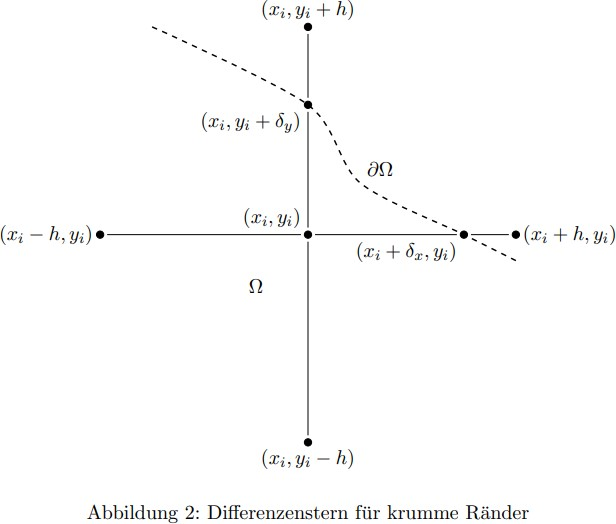
\includegraphics{Abbildung_2}
\end{exercise}

\begin{solution}
  Beweis.
\end{solution}

\begin{algebraUE}{397}
Sei $p \in \P$ eine Primzahl. Zeigen Sie, dass $GF(p^{\infty})$ überabzählbar viele
nichtisomorphe Unterkörper hat. \\
\textit{Anleitung:} Für jede (unendliche) Menge $A \subseteq \P$ sei $K_A$ Vereinigung
aller $GF(p^n)$, für die gilt, dass alle Primfaktoren von $n$ in $A$ liegen.
Schreiben Sie $K_A$ als aufsteigende Vereinigung $\bigcup_{j=1}^{\infty}U_j$
von Unterkörpern, um zu beweisen, dass $K_A$ ein Körper ist. Für $A \neq A^{\prime}$
zeigen Sie $K_A \ncong K_{A^\prime}$, indem Sie ein Polynom (wo liegen die
Koeffizienten dieses Polynoms?) finden, das zwar in $K_A$, aber nicht in $K_{A^{\prime}}$
eine Nullstelle hat, oder umgekehrt.
\end{algebraUE}

\begin{solution}

ToDo!

\end{solution}

% --------------------------------------------------------------------------------

\begin{exercise}[270]

Sei $g: M \to M$ injektiv, aber nicht surjektiv. Geben Sie (in Abhängigkeit von $g$)
explizit eine injektive Abbildung $f: \N \to M$ an.
(Genauer: Geben Sie eine explizite Familie $(f_a: a \in I)$ von solchen Abbildungen
an, mit $I \neq \emptyset$.)

\end{exercise}

% --------------------------------------------------------------------------------

\begin{solution}

Weil $g$ nicht surjektiv ist, ist $I := M \setminus g[M] \neq \emptyset$.
Sei also $a \in I$.

\begin{align*}
    f_a:
    \N \to M:
    n
    \mapsto
	\begin{cases}
		a,             & \text{falls}~ n = 0, \\
		g(f_a(n - 1)), & \text{falls}~ n > 0 
	\end{cases}
\end{align*}

Wir wollen nun folgende Aussage, d.h. die Injektivität von $f_a$, mit Induktion nach $n$ beweisen.

\begin{align*}
    \Forall n, k \in \N:
    (f_a(k) = f_a(n) \implies k = n)
\end{align*}

IA ($n = 0$):
Sei $k \in \N$ mit $f_a(0) = f_a(n) = f_a(k)$.
Angenommen, $k \neq 0$, d.h. $k > 0$.

\begin{align*}
    \implies
    m = f_a(0) = f_a(k) = g(f_a(k - 1))
    \implies
    m \in g[M]
\end{align*}

Widerspruch!

IS ($n \mapsto n + 1$):
Für $n \in \N$ gelte bereits

\begin{align*}
    \Forall k \in \N:
    (f_a(n) = f_a(k) \implies n = k).
\end{align*}

Sei $k \in \N$ mit $f_a(n + 1) = f_a(k)$.
Wäre $k = 0$, dann würde wegen $n + 1 > 0 = k$, mit dem IA ($k = 0$) ein Widerspruch folgen.

\begin{align*}
    \implies
	g(f_a(n)) = f_a(n + 1) = f_a(k) = g(f_a(k - 1))
\end{align*}

Wegen der Injektivität von $g$, folgt $f_a(n) = f_a(k - 1)$.
Wegen der Induktionsvoraussetzung, folgt außerdem $n = k - 1$ und daher $n + 1 = k$. 

\end{solution}


\end{document}
